\section{Results}\label{sect:results}
The subvolumes associated with the zonal anatomy in each imaging modality were
measured (Figure~\ref{fig:mr_arfi_volumes}(a)), with moderate correlation
between the ARFI and MR total prostate gland volumes (R$^2$ = 0.63), with a
mean overestimation of of 6.1 $\pm$ 25.0\% by ARFI imaging compared to MR
volumes (Figure~\ref{fig:mr_arfi_volumes}(b)).  Central gland volumes were
slightly less correlated between ARFI and MR images (R$^2$ = 0.38) with no
significant mean over/under-estimation (-5.0 $\pm$ 39.5\%), but significant
variability between the cases (Figure~\ref{fig:mr_arfi_volumes}(c)).
Table~\ref{tab:mr_arfi_volumes} has the individually-measured volumes for MR
and ARFI imaging for each study subject.

\begin{figure}[htb!]
\centering
\begin{tabular}{ccc}
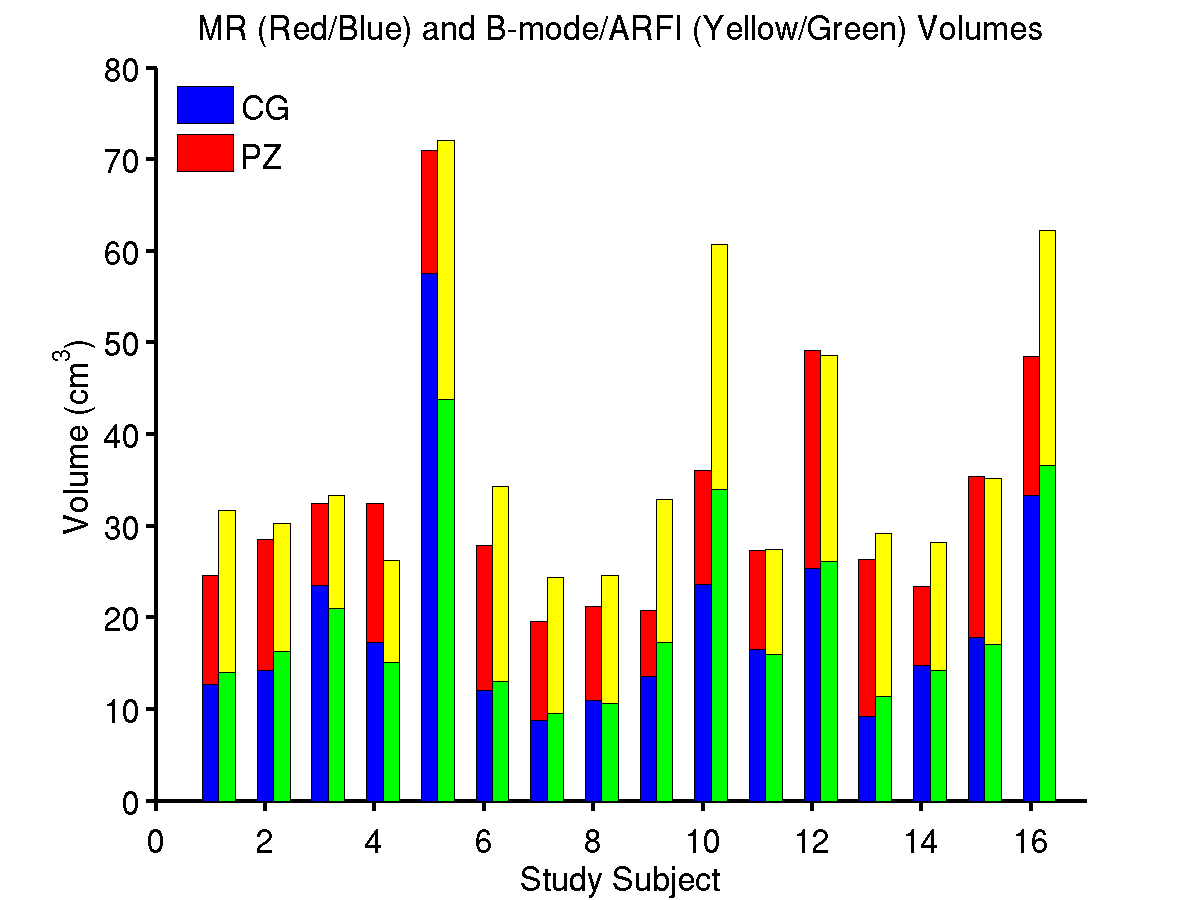
\includegraphics[width=0.3\linewidth]{figs/mr_arfi_volumes} &
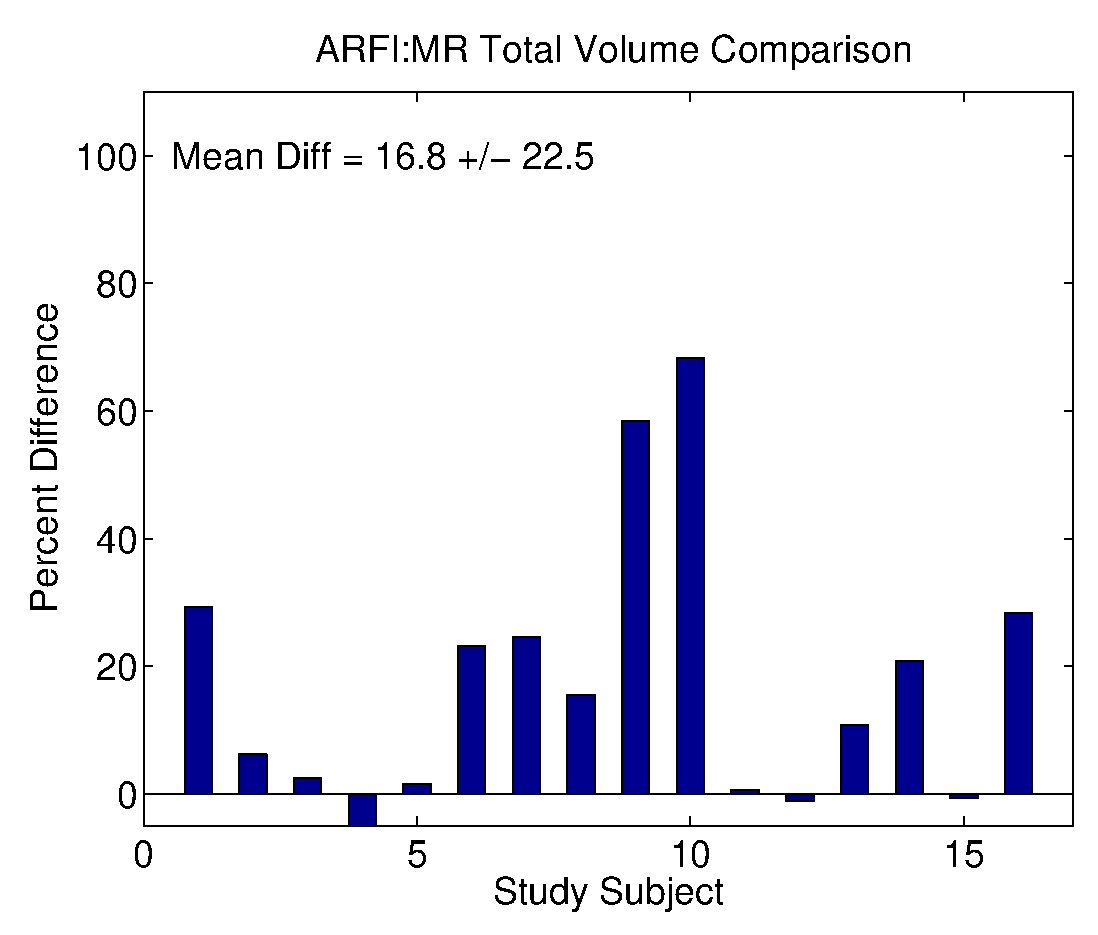
\includegraphics[width=0.3\linewidth]{figs/mr_arfi_volume_diff} &
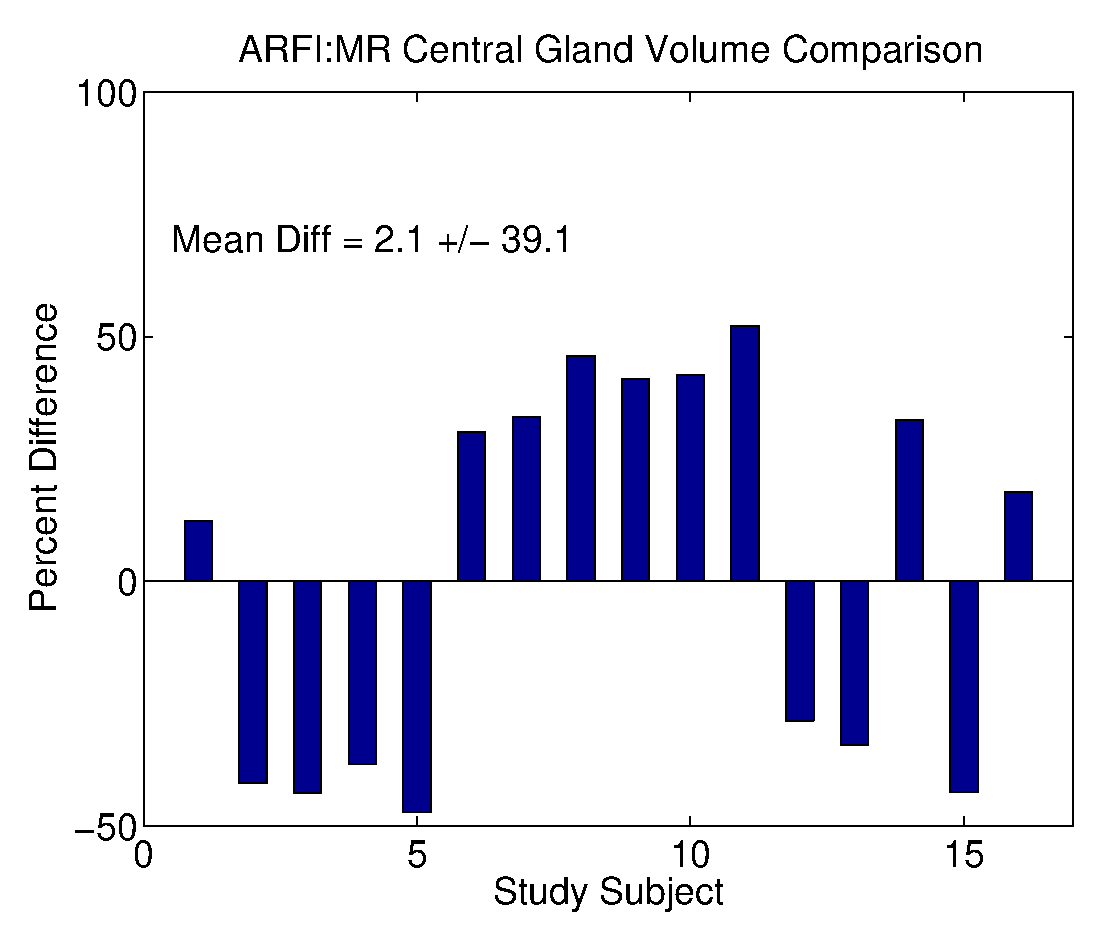
\includegraphics[width=0.3\linewidth]{figs/mr_arfi_central_diff} \\
(a) Central:Peripheral Volume & (b) Total Volume Difference & (c) Central Volume Difference\\
\end{tabular}
\caption{Comparison of MR and ARFI zonal anatomy volume estimates from
    manually-segmented images.  Total prostate volumes ranged from 19.6--71.0
    cm$^3$ based on MR image models (a), with ARFI image models overestimating
    total prostate volume by 36.7 $\pm$ 27.9\% (b).  ARFI image estimation of
    the central zone volume relative to the MR central gland volume varied by
    2.1 $\pm$ 39.0\% (c).  Table~\ref{tab:mr_arfi_volumes} contains the
    individual volume estimates for the entire prostate and the central
    glands.}
\label{fig:mr_arfi_volumes} 
\end{figure}


Weights and axis measurements from the gross pathology processing of the
excised prostates were collected (Table~\ref{tab:path_data}), and using the
axis measurements (lateral-to-lateral, anterior-to-posterior, and
apex-to-base), the prostate volume was approximated as a tri-axial ellipsoid,
and its volume was estimated (\ref{eqn:ellipsoid_volume}).  Prostate weights
were moderately correlated with estimated pathology ellipsoidal prostate
volumes (Figure~\ref{fig:mr_arfi_weight}(a), R$^2$ = 0.68).  There was moderate
correlation between the prostate weight and the image-reconstructed prostate
volumes (Figure~\ref{fig:mr_arfi_weight}(b), R$^2$ = 0.44 (MR) and 0.18
(ARFI)), though there was weaker correlation with the ellipsoidal approximation
of the measurement prostate volume and the image-reconstructed volumes
(Figure~\ref{fig:mr_arfi_weight}(c), R$^2$ = 0.08 (MR) and 0.00 (ARFI)).  

\begin{figure}[htb!]
\centering
\begin{tabular}{lll}
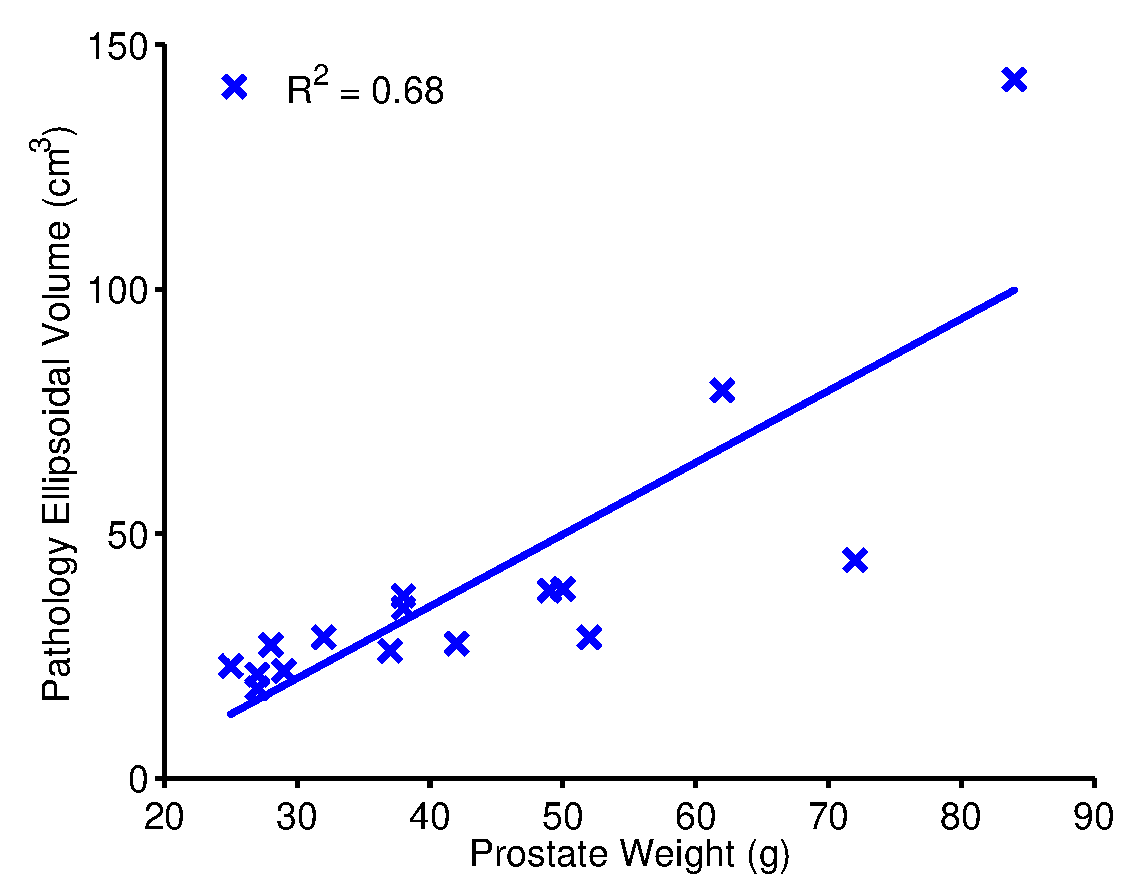
\includegraphics[width=0.3\linewidth]{figs/corr_path_vol_weight_vol} &
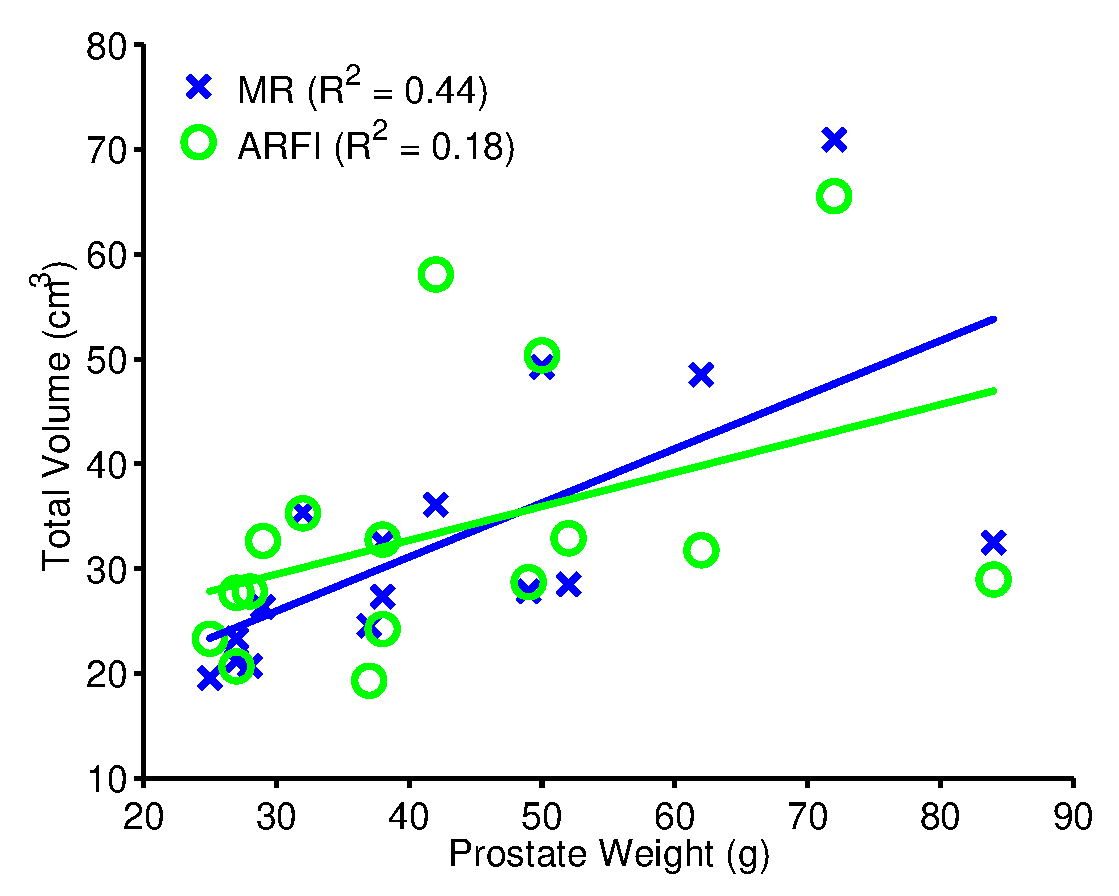
\includegraphics[width=0.3\linewidth]{figs/corr_weight_vol} &
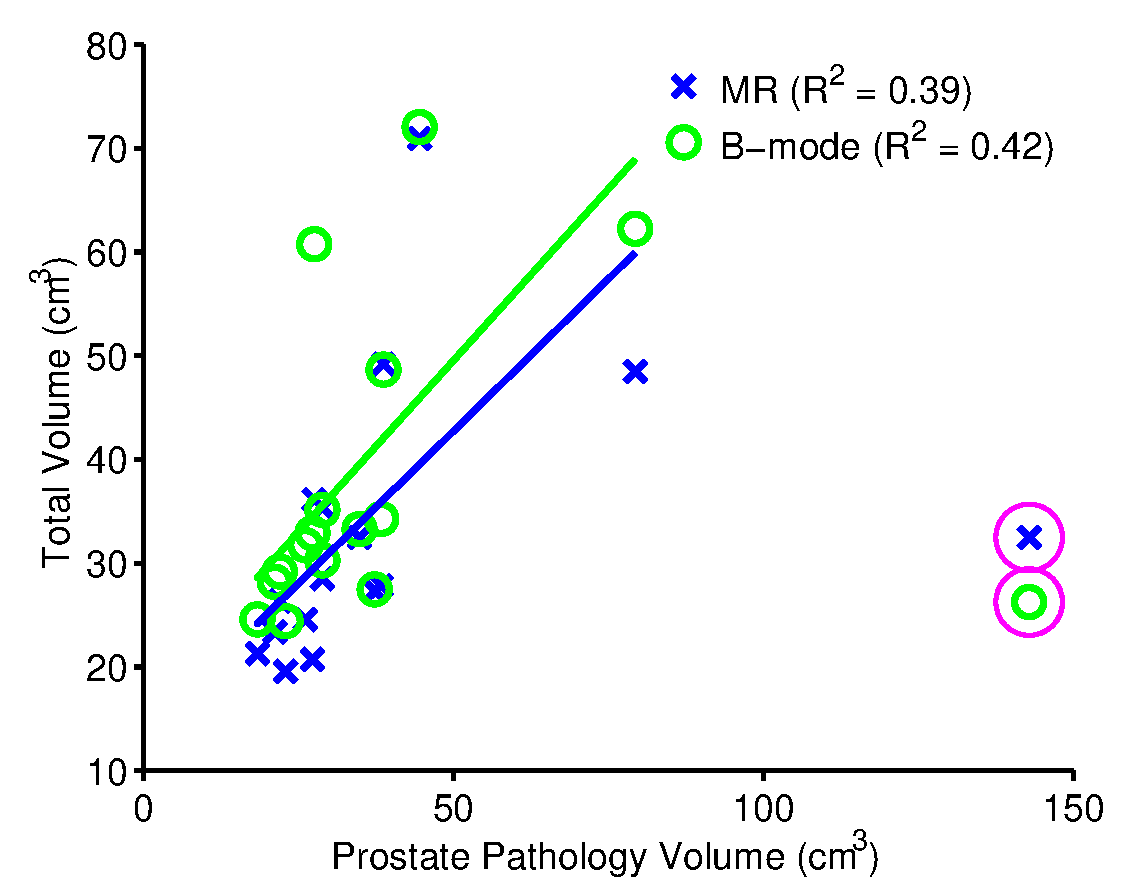
\includegraphics[width=0.3\linewidth]{figs/corr_pathVol_vol} \\
(a) Path Weight : Path Volume & (b) Image Volume : Prostate Weight & (c) Image Volume : Path Volume \\
\end{tabular}
%\begin{tabular}{ll}
%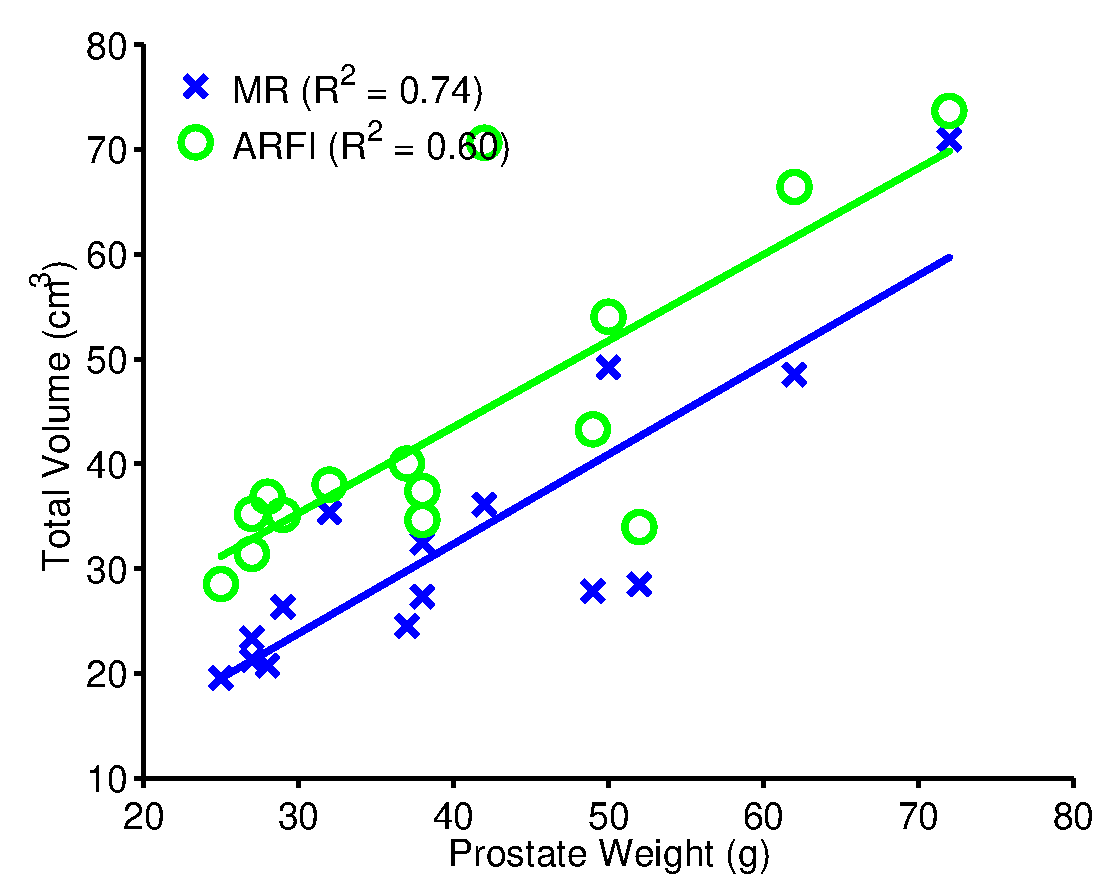
\includegraphics[width=0.3\linewidth]{figs/corr_weight_vol_no4} &
%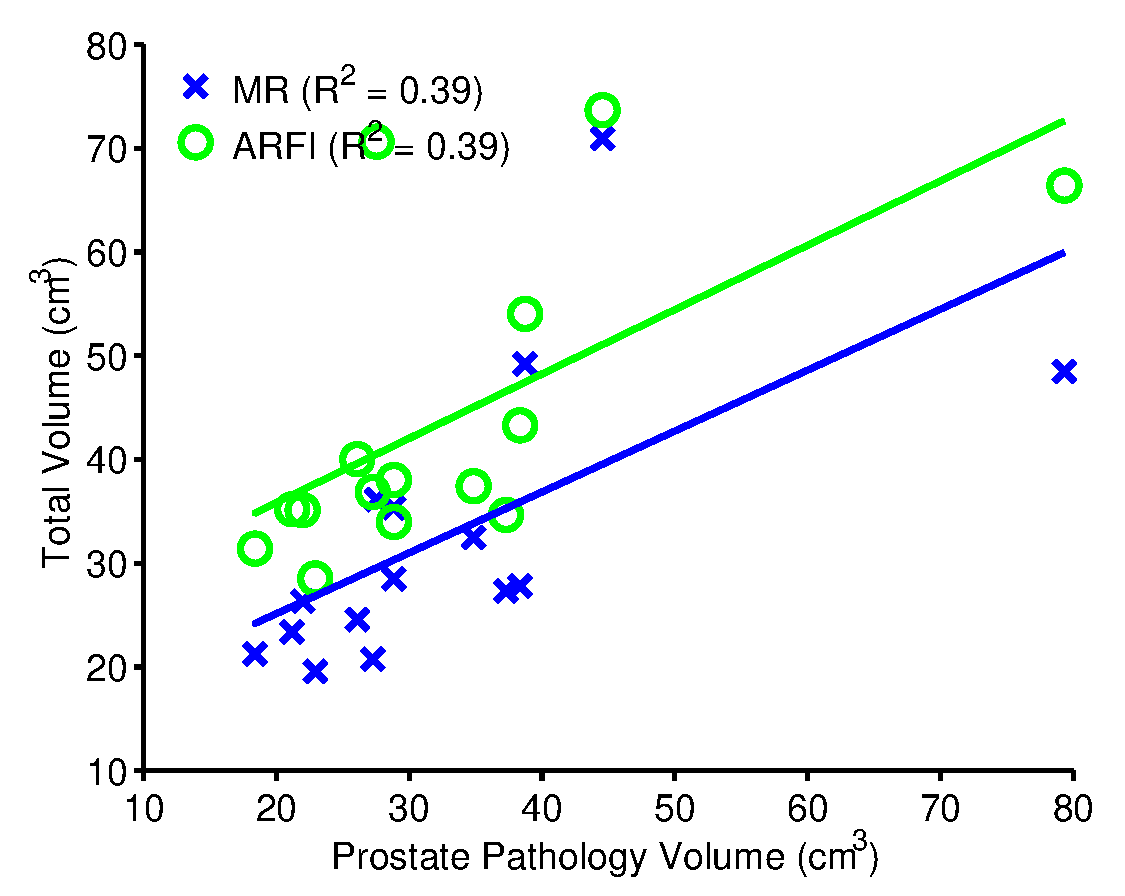
\includegraphics[width=0.3\linewidth]{figs/corr_pathVol_vol_no4} \\
%(d) Image Volume : Prostate Weight (-4) & (e) Image Volume : Path Volume (-4) \\
%\end{tabular}
\caption{Tri-axial pathology measurements were used to make an ellipsoidal
    prostate volume approximation based on gross pathology axis measurements,
    which was moderately well-correlated with the excised prostated weights (a,
    R$^2$ = \pathVolWeightRsq).  T2WI MR (blue, X) showed a moderate
    correlation between the reconstructed volumes and prostate weight (R$^2$ =
    \weightMRrsq), while volumes reconstructed from ARFI images (green, O)
    showed weaker correlation (R$^2$ = \weightARFIrsq) (b).  Weaker
    correlations existed between both T2WI MR and ARFI image volumes and
    approximated ellipsoidal prostate pathology volumes (R$^2$ = \pathVolMRrsq
    and \pathVolARFIrsq, respectively) (c).  One study subject had a very large
    prostate ($>$ 80 g) that was not well visualized by both MR and ARFI
    imaging, and it was excluded from all of the linear regression.  This
    outlier was indicated with magenta circles in the plots.}
\label{fig:mr_arfi_weight}
\end{figure}


Measurements of the prostate total and CG dimensions along the three
standard anatomic axes (apex-to-base, lateral-to-lateral, and
anterior-to-posterior) were made (Table~\ref{tab:mr_arfi_axes}), and the
correlation between the imaging axis measurements was analyzed
(Figure~\ref{fig:mr_arfi_path_axes}).  ARFI was most correlated to MR in the
lateral-to-lateral axis in both the total and CG (R$^2$ = 0.57 and
0.32, respectively), with mean overestimates of 13.5 $\pm$ 11.0\% and 11.5 $\pm$
22.5\%, respectively (Table~\ref{tab:mr_arfi_axes_error}).  ARFI had moderate
correlation with the total prostate gland axis in the anterior-to-posterior
dimension (R$^2$ = 0.23), but poor correlation in the CG (R$^2$ =
0.00), with overestimates of 5.7 $\pm$ 20.6 and -8.4 $\pm$ 24.0\%.  ARFI
imaging had weak correlation with MR images in the apex-to-base dimension
(R$^2$ = 0.19, total gland and R$^2$ = 0.09, CG), with differences
of -2.4 $\pm$ 17.0 and 1.2 $\pm$ 19.8\%, respectively.

\begin{figure}
\centering
\begin{tabular}{ccc}
%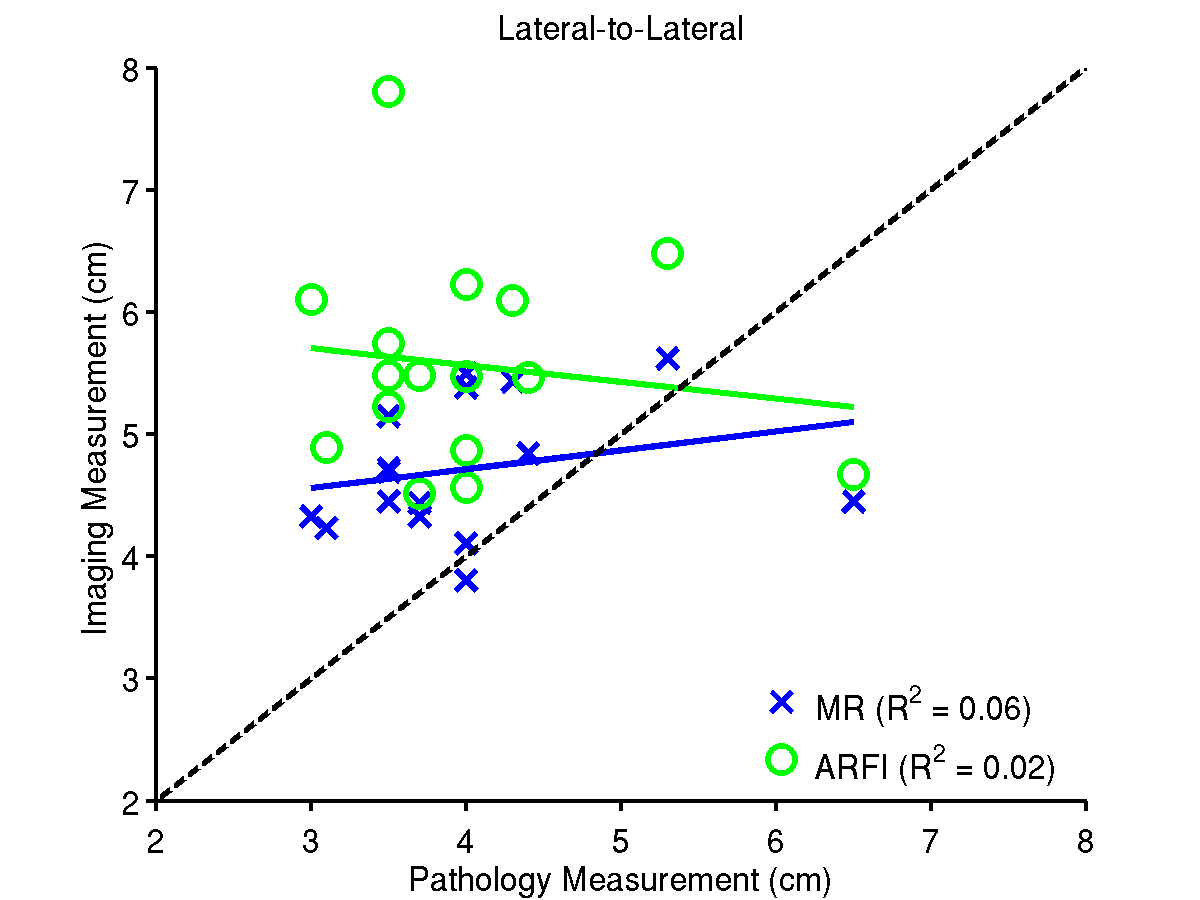
\includegraphics[width=0.3\linewidth]{figs/Lateral-to-Lateral} &
%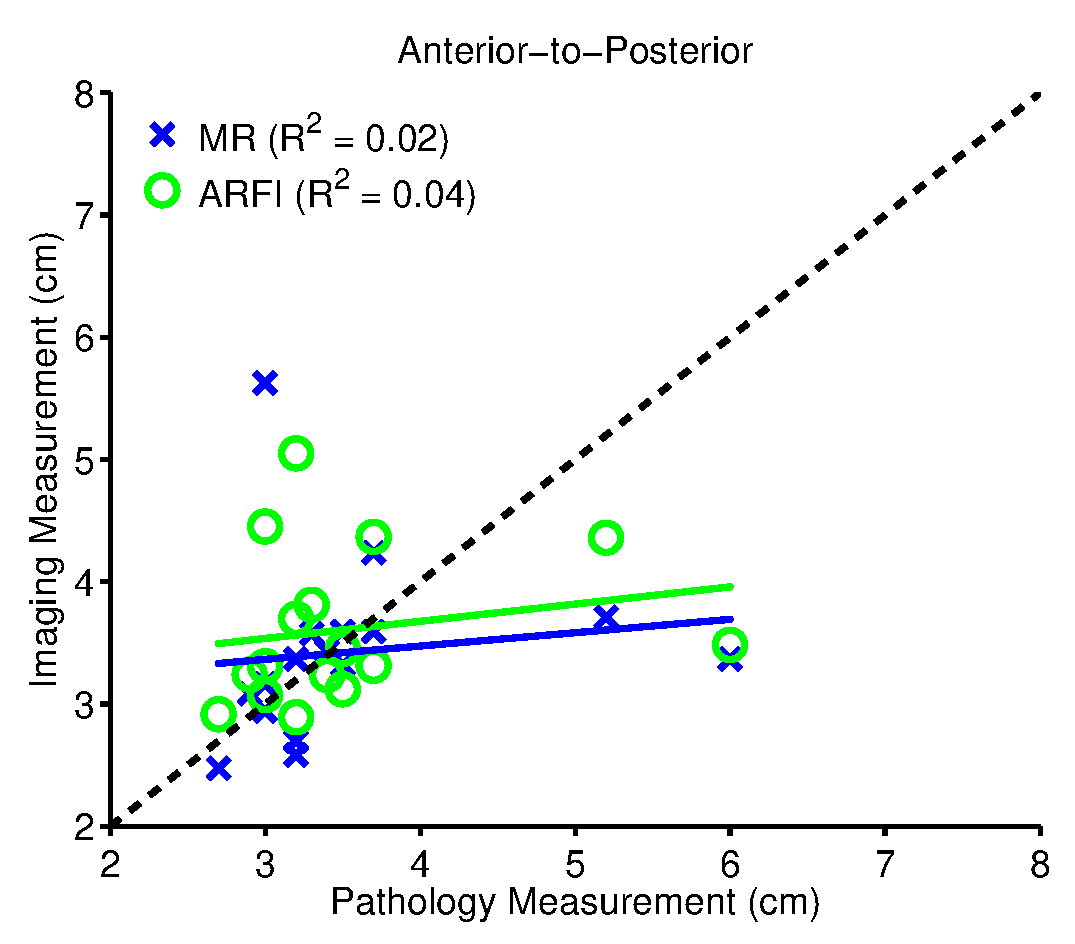
\includegraphics[width=0.3\linewidth]{figs/Anterior-to-Posterior} &
%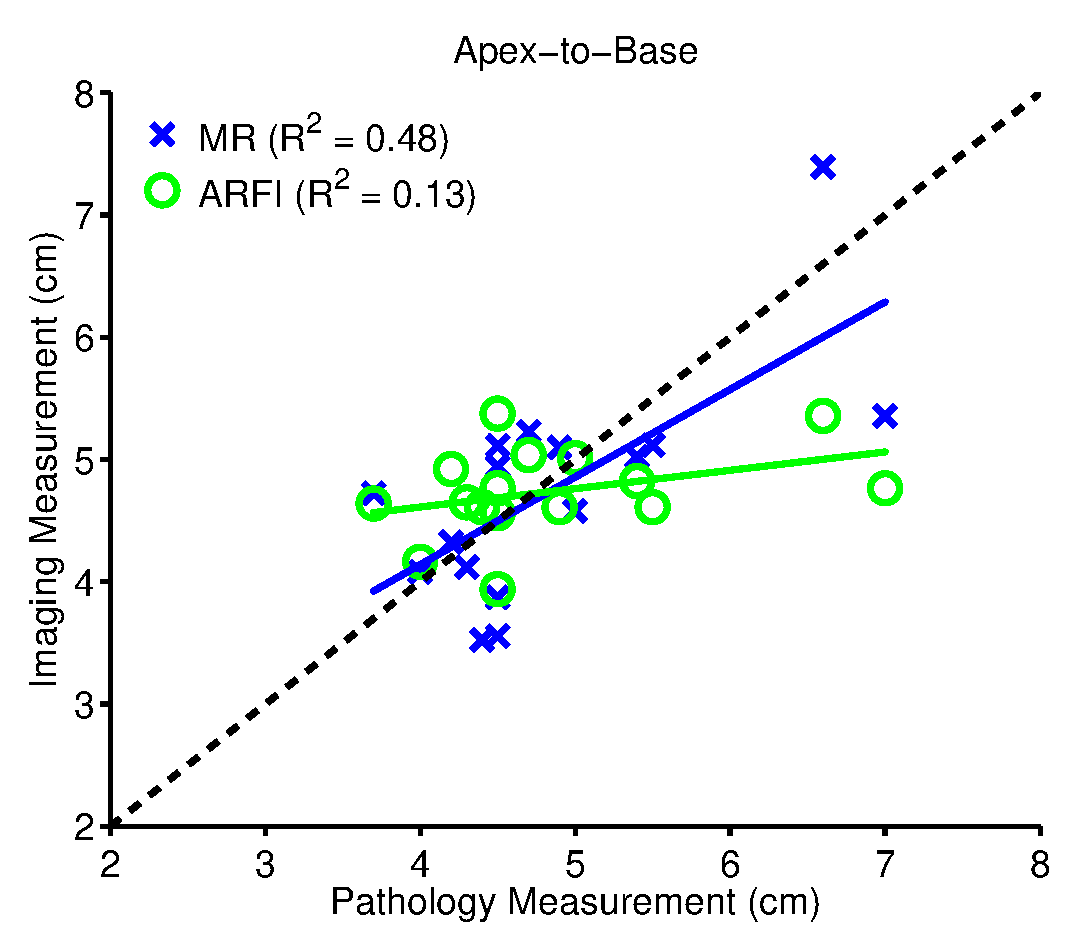
\includegraphics[width=0.3\linewidth]{figs/Apex-to-Base} \\
%(a) & (b) & (c) \\
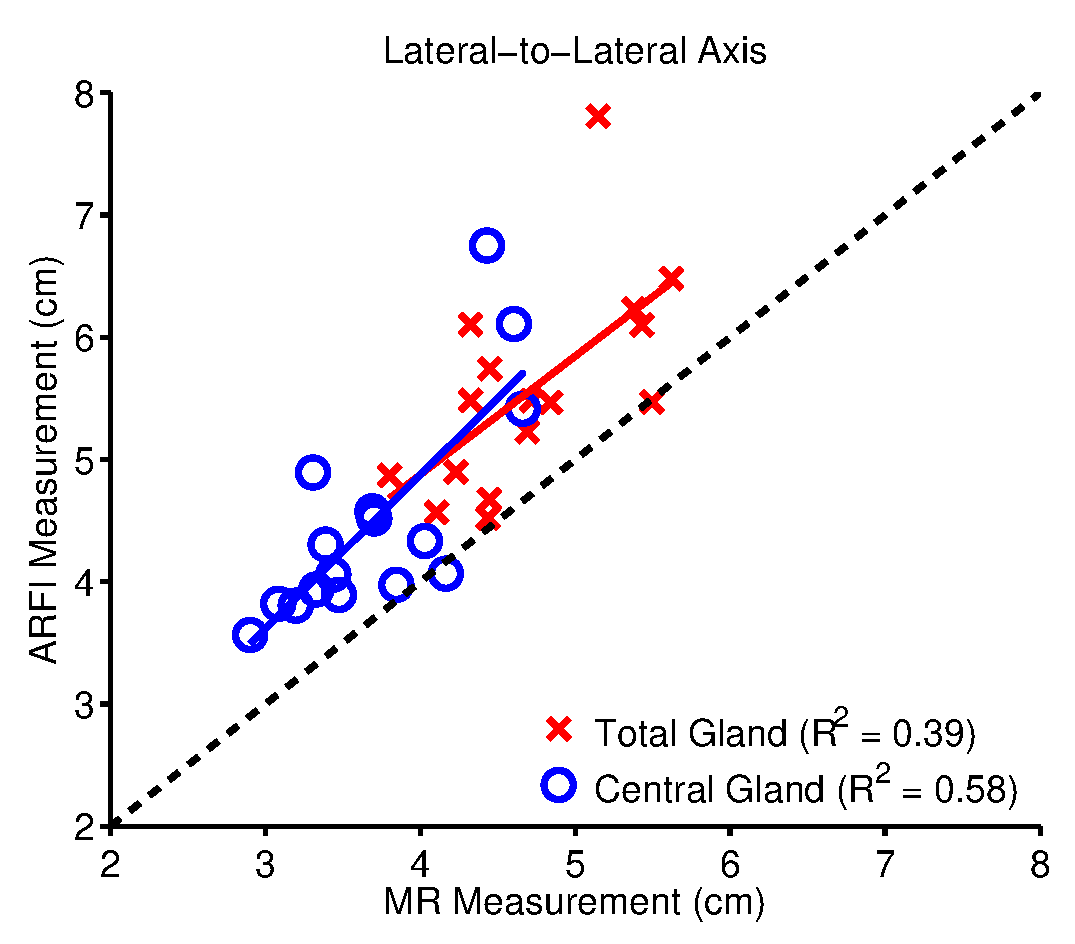
\includegraphics[width=0.3\linewidth]{figs/Imaging_Lateral-to-Lateral} &
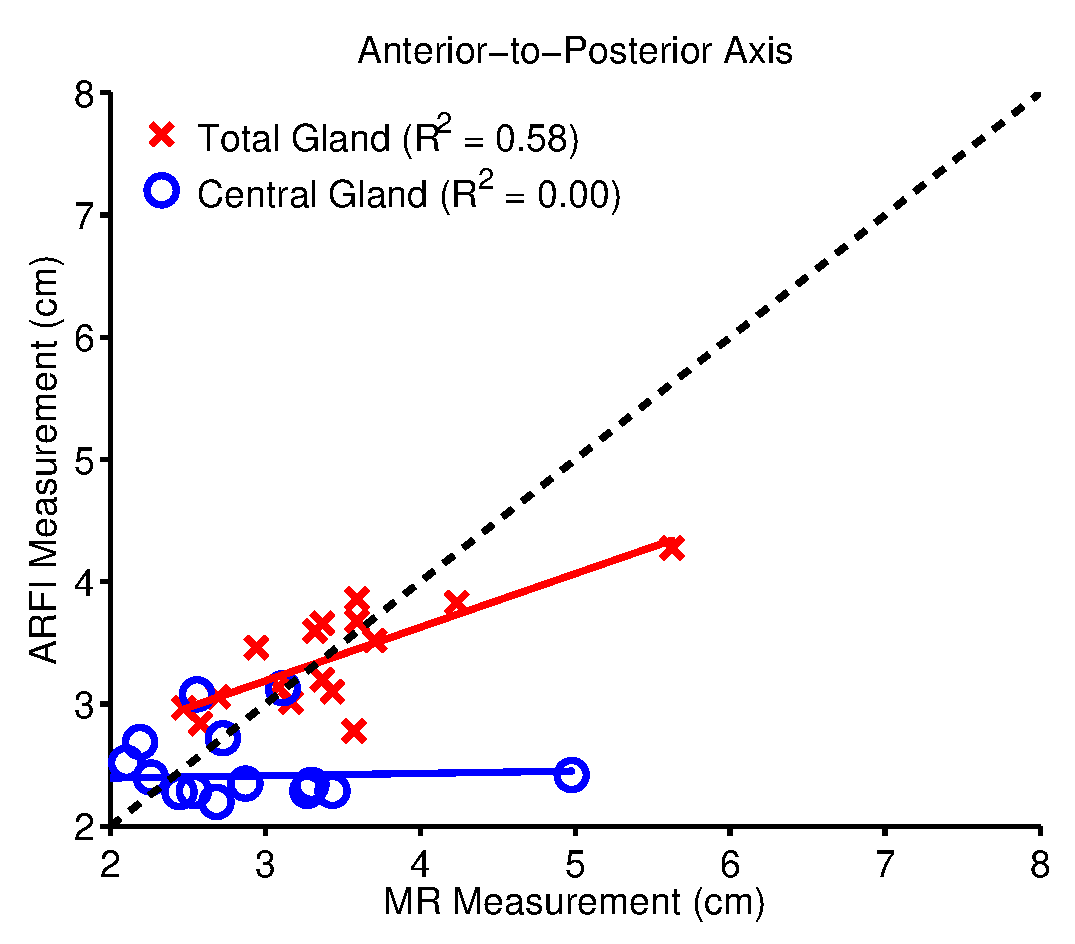
\includegraphics[width=0.3\linewidth]{figs/Imaging_Anterior-to-Posterior} &
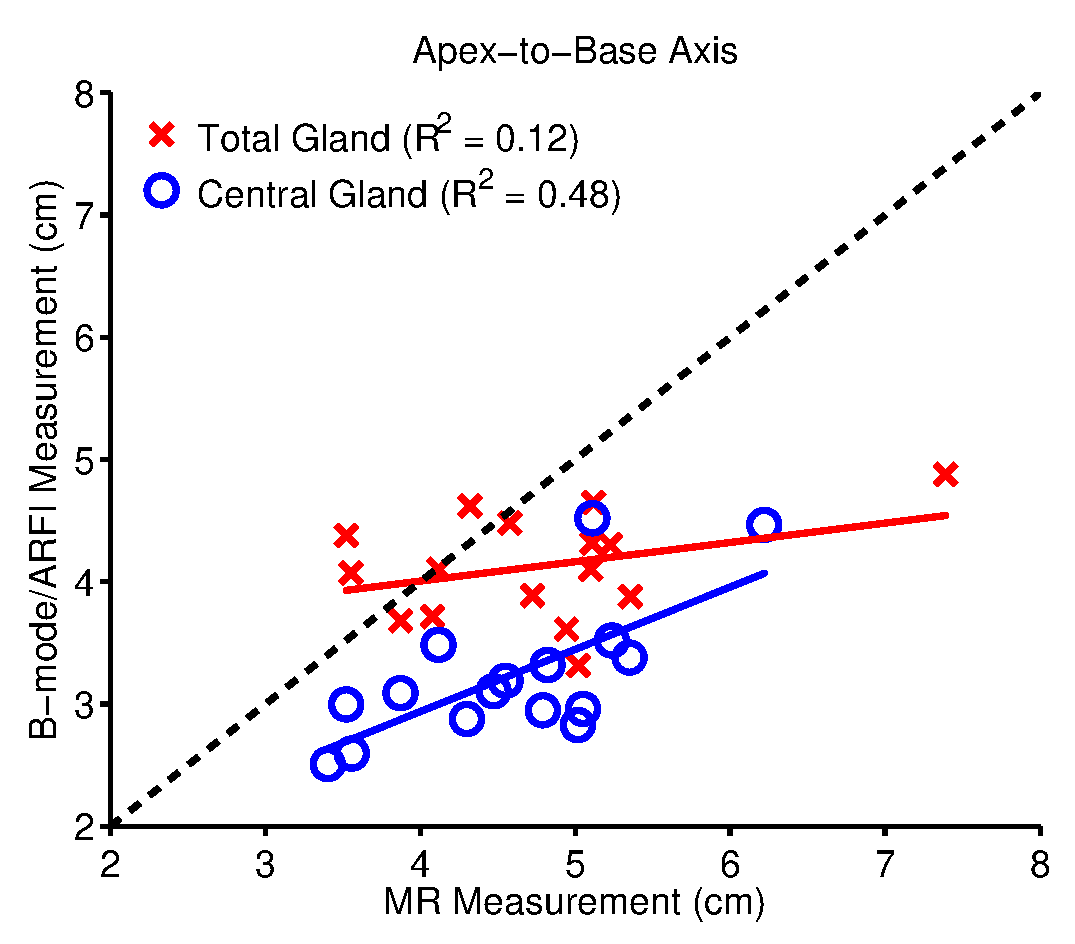
\includegraphics[width=0.3\linewidth]{figs/Imaging_Apex-to-Base} \\
(a) & (b) & (c) \\
%(d) & (e) & (f) \\
\end{tabular}
\caption{Measurements of the prostate dimensions along the three standard
    anatomic axes: lateral-to-lateral (a), anterior-to-posterior (b) and
    apex-to-base (c).  The correlation between the MR and B-mode/ARFI imaging
    axis measurements was performed in each orientation for the total gland
    (red crosses) and central gland (blue circles).  \textbf{B-mode images were
        used for total gland measurements, and ARFI images were for central
        gland measurements.} The black dashed-line represents the projection of
    perfectly-correlated measurements between imaging and pathology.  The
    over-/under-estimation of each imaging modality relative to gross pathology
    and each other is summarized in Table~\ref{tab:mr_arfi_axes_error}.} 
\label{fig:mr_arfi_path_axes}
\end{figure}


\begin{table}[h!]
\centering
\caption{Difference in ARFI imaging axis measurements relative to MR T2WI measurements.}
\begin{tabular}{|l|l|l|} \hline
 & {\bf ARFI:MR} & {\bf ARFI:MR} \\
 & {\bf Total Gland (\%)} & {\bf Central Gland (\%)} \\ \hline
{\bf Lateral-to-Lateral} & 8.1 $\pm$ 18.4 & 0.06 $\pm$ 17.2 \\
{\bf Anterior-to-Posterior} & 17.0 $\pm$ 12.1 & 14.8 $\pm$ 23.1 \\
{\bf Apex-to-Base} & 0.58 $\pm$ 12.9 & -10.8 $\pm$ 22.3 \\
\hline
\end{tabular}
\label{tab:mr_arfi_axes_error}
\end{table}


%\begin{figure}
\centering
\begin{tabular}{ccc}
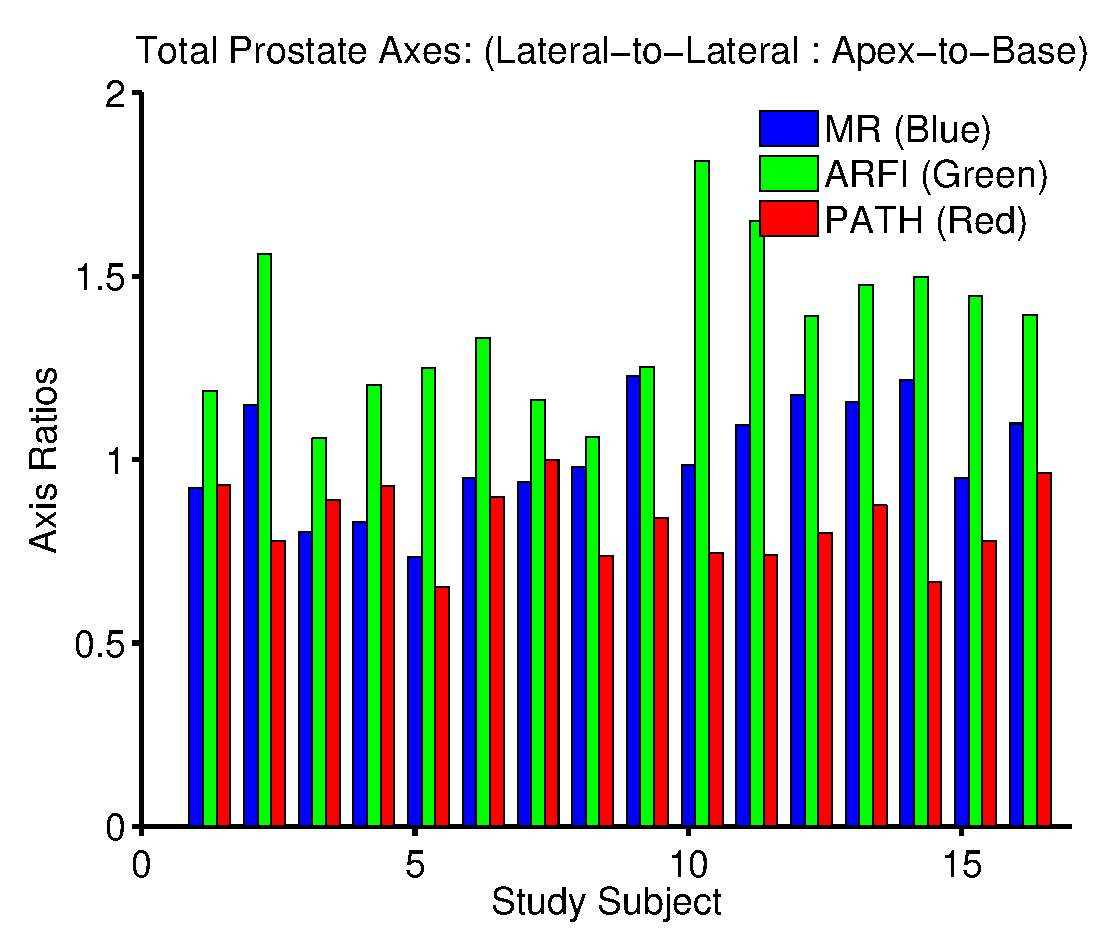
\includegraphics[width=0.3\linewidth]{figs/mr_arfi_total_axes1} &
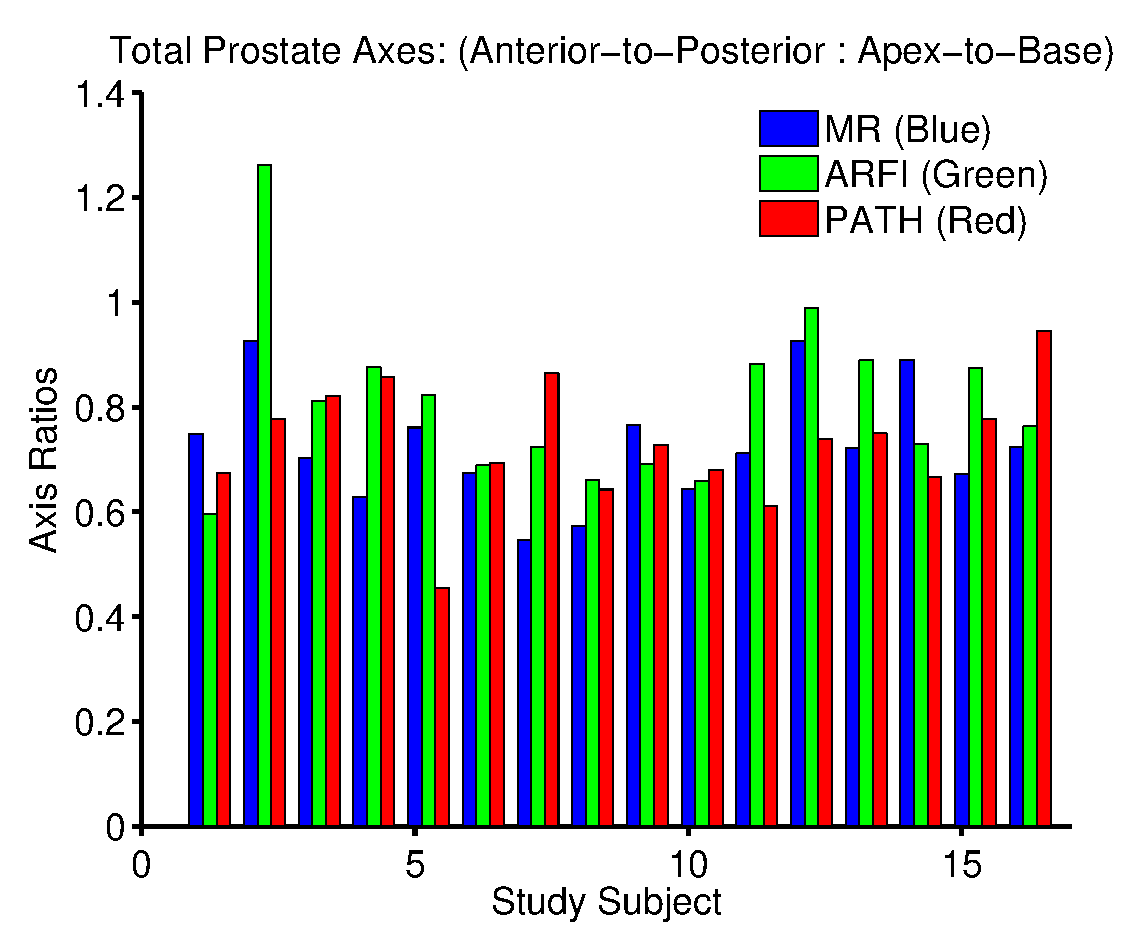
\includegraphics[width=0.3\linewidth]{figs/mr_arfi_total_axes2} &
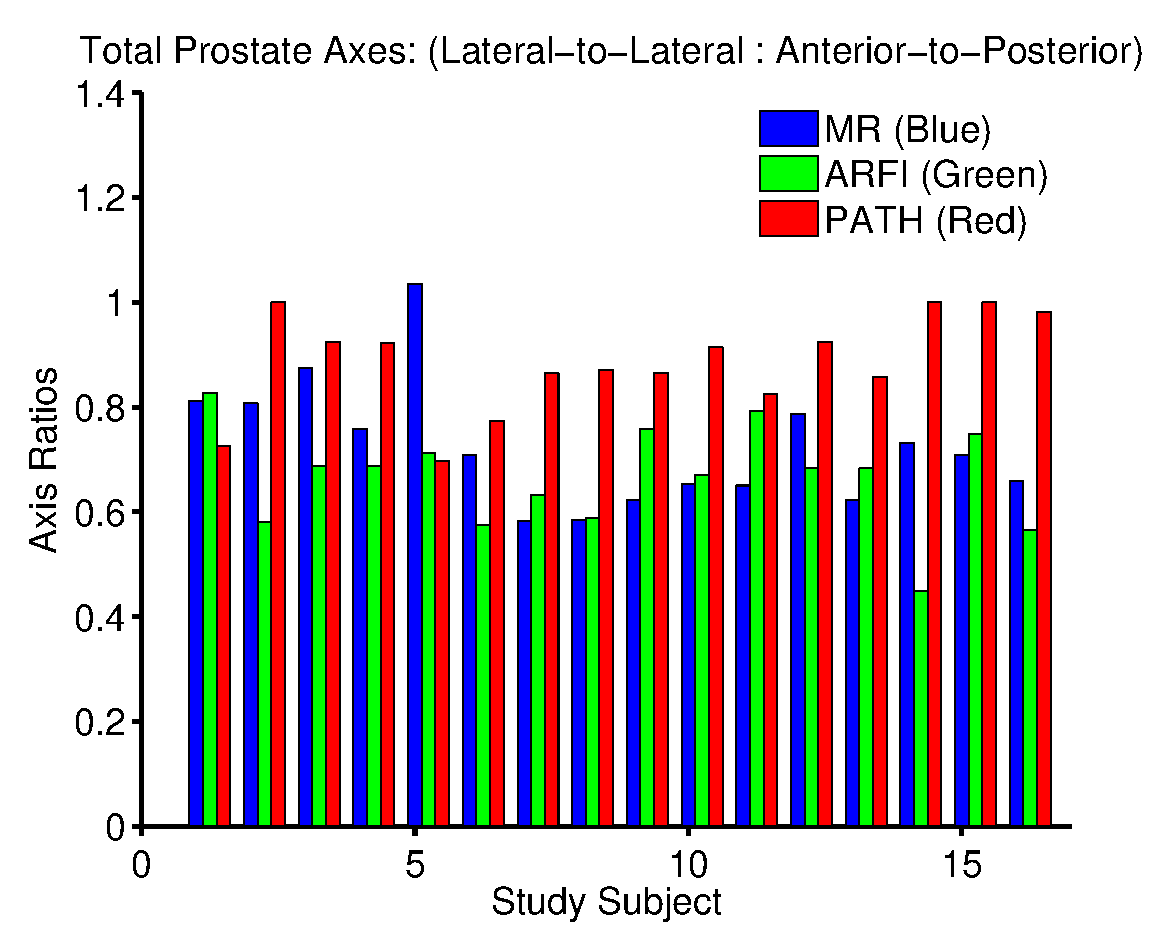
\includegraphics[width=0.3\linewidth]{figs/mr_arfi_total_axes3} \\
(a) & (b) & (c) \\
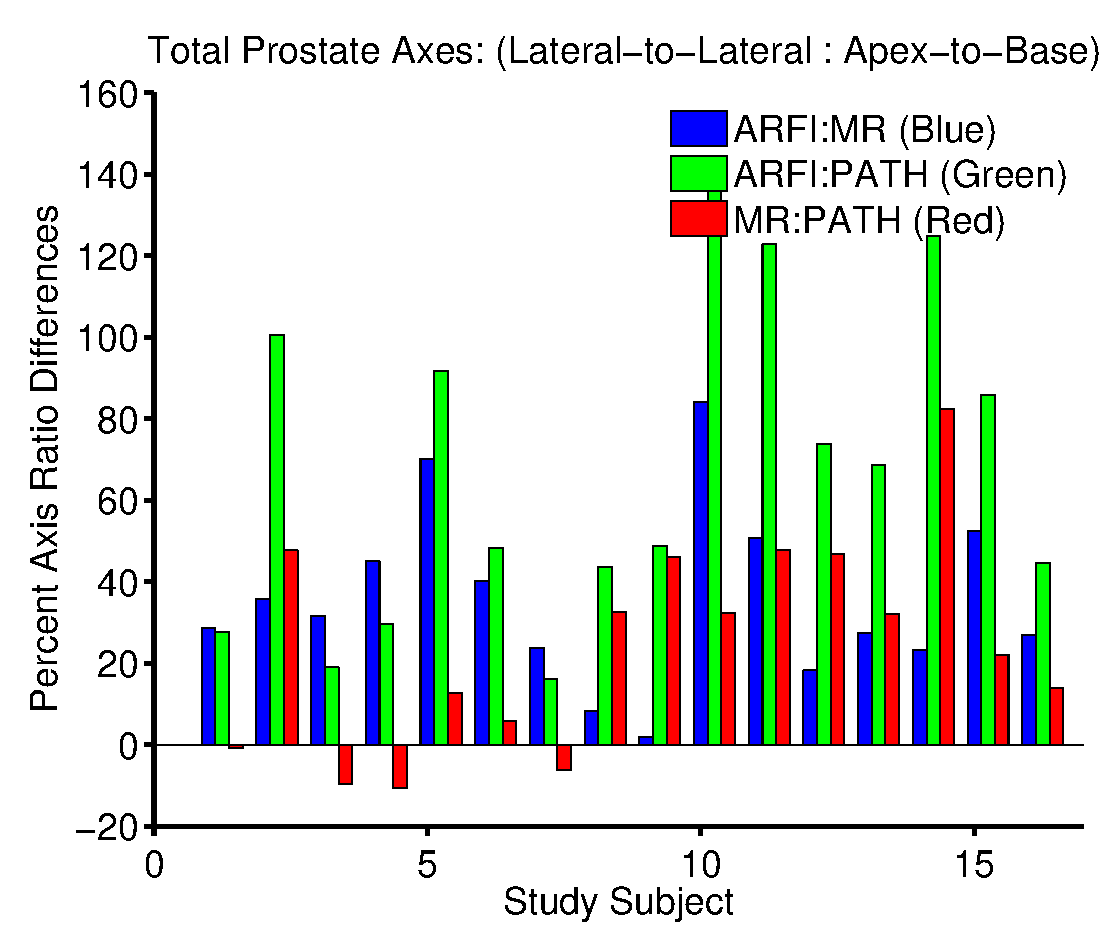
\includegraphics[width=0.3\linewidth]{figs/mr_arfi_total_over_under1} &
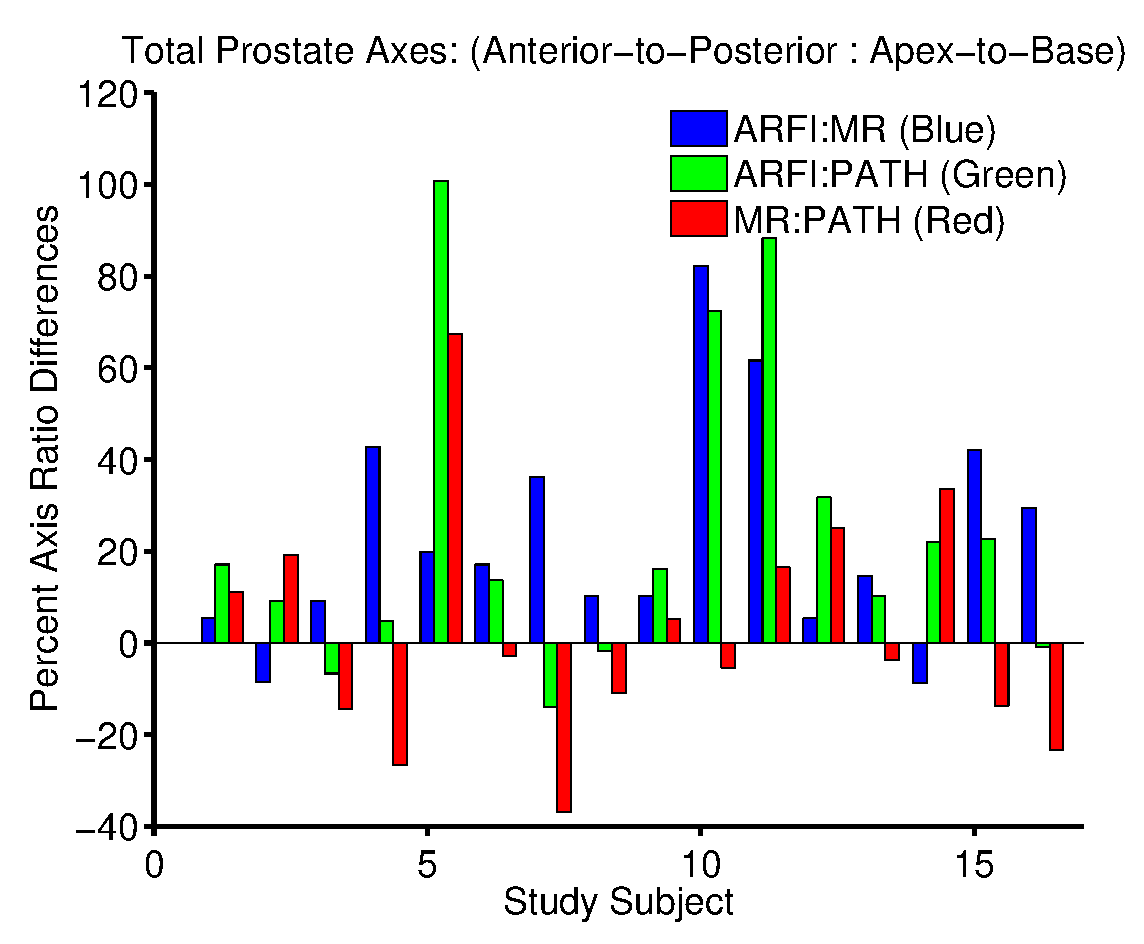
\includegraphics[width=0.3\linewidth]{figs/mr_arfi_total_over_under2} &
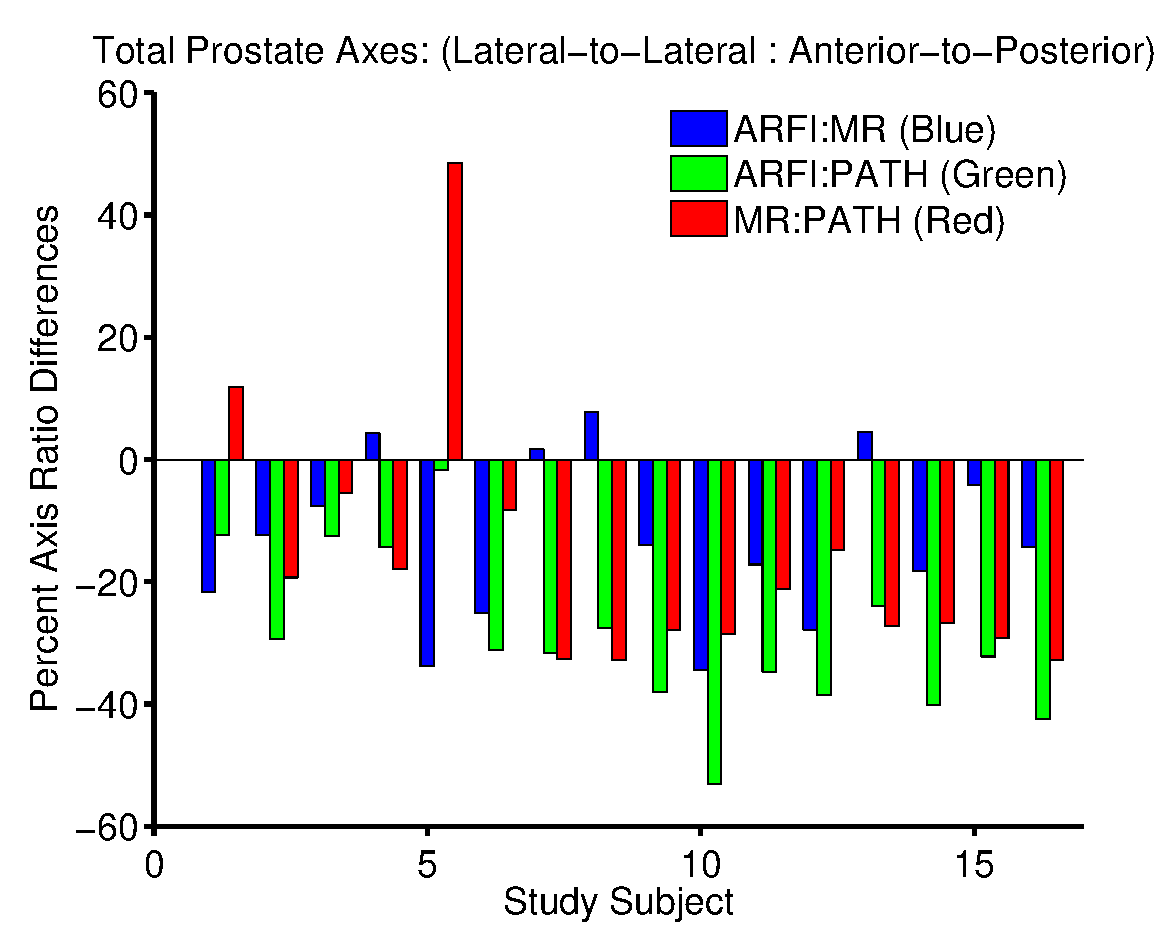
\includegraphics[width=0.3\linewidth]{figs/mr_arfi_total_over_under3} \\
(d) & (e) & (f) \\
\end{tabular}
\caption{Comparison of the ratios of the three anatomic axis measurement ratios
    for T2WI MR (top row, blue), ARFI imaging (top row, green) and gross
    pathology (top row, red).  The over/underestimation of the axis ratios
    between ARFI imaging : T2WI MR : Pathology are shown in the bottom row
    (d-f), with mean ratio differences compiled in
    Table~\ref{tab:axis_ratio_over_under}.}
\label{fig:mr_arfi_total_axes} 
\end{figure}


%\begin{figure}
\centering
\begin{tabular}{ccc}
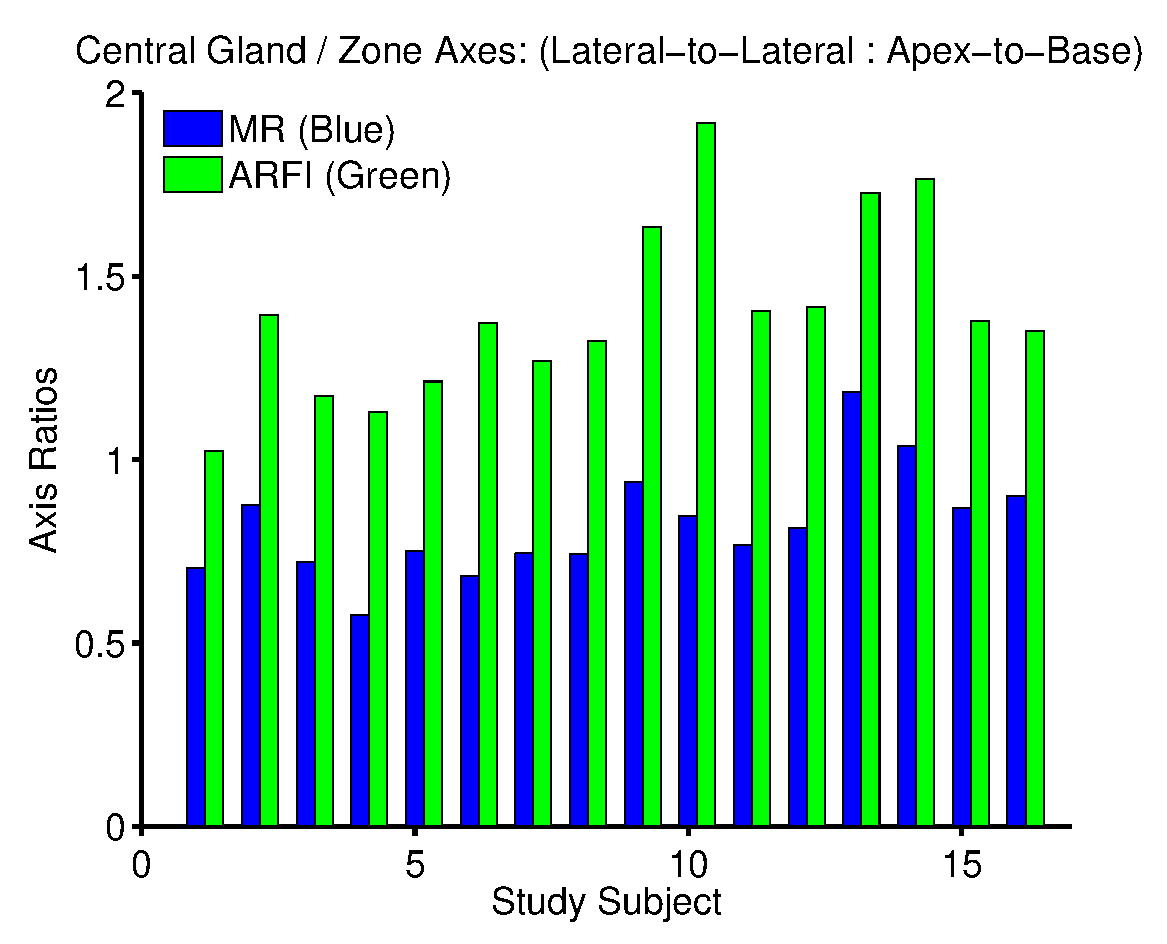
\includegraphics[width=0.3\linewidth]{figs/mr_arfi_central_axes1} &
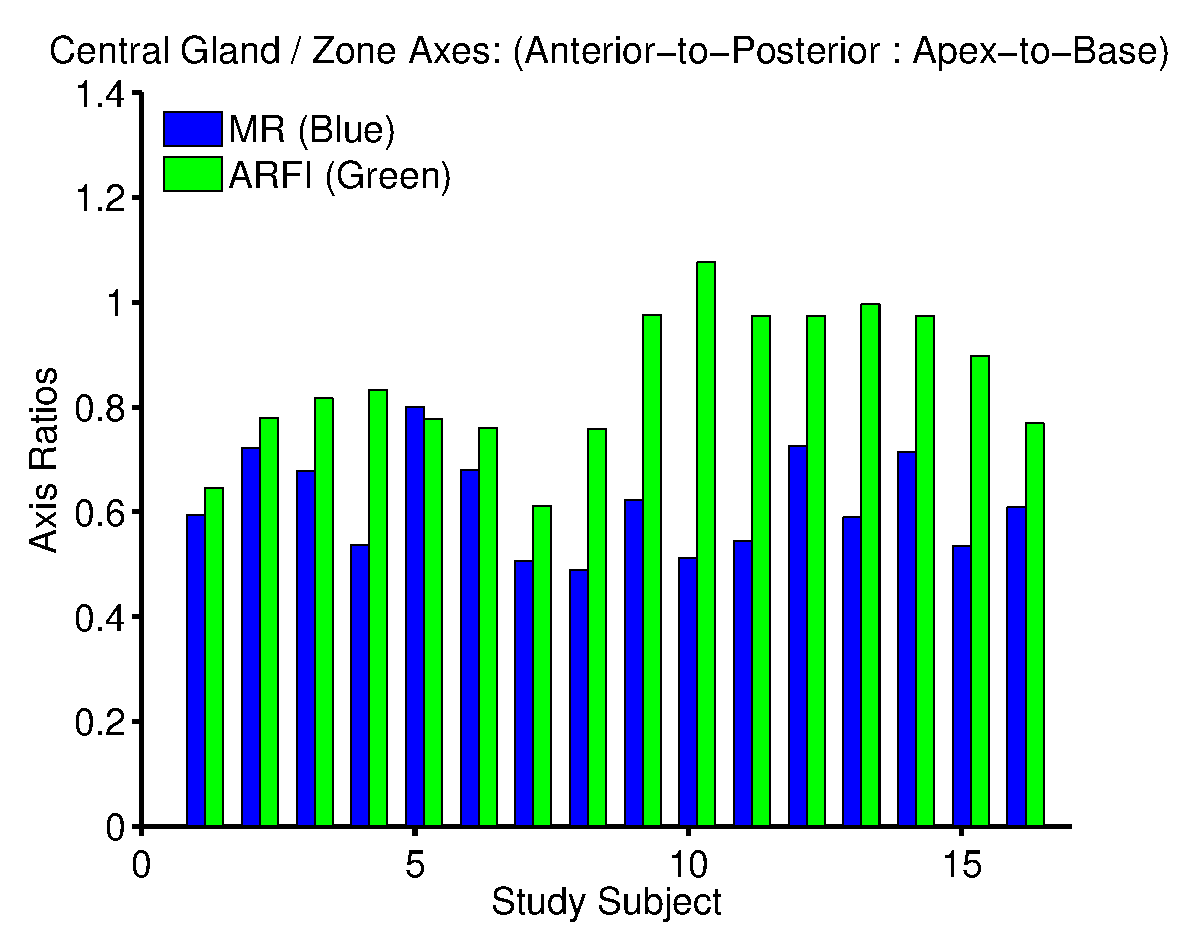
\includegraphics[width=0.3\linewidth]{figs/mr_arfi_central_axes2} &
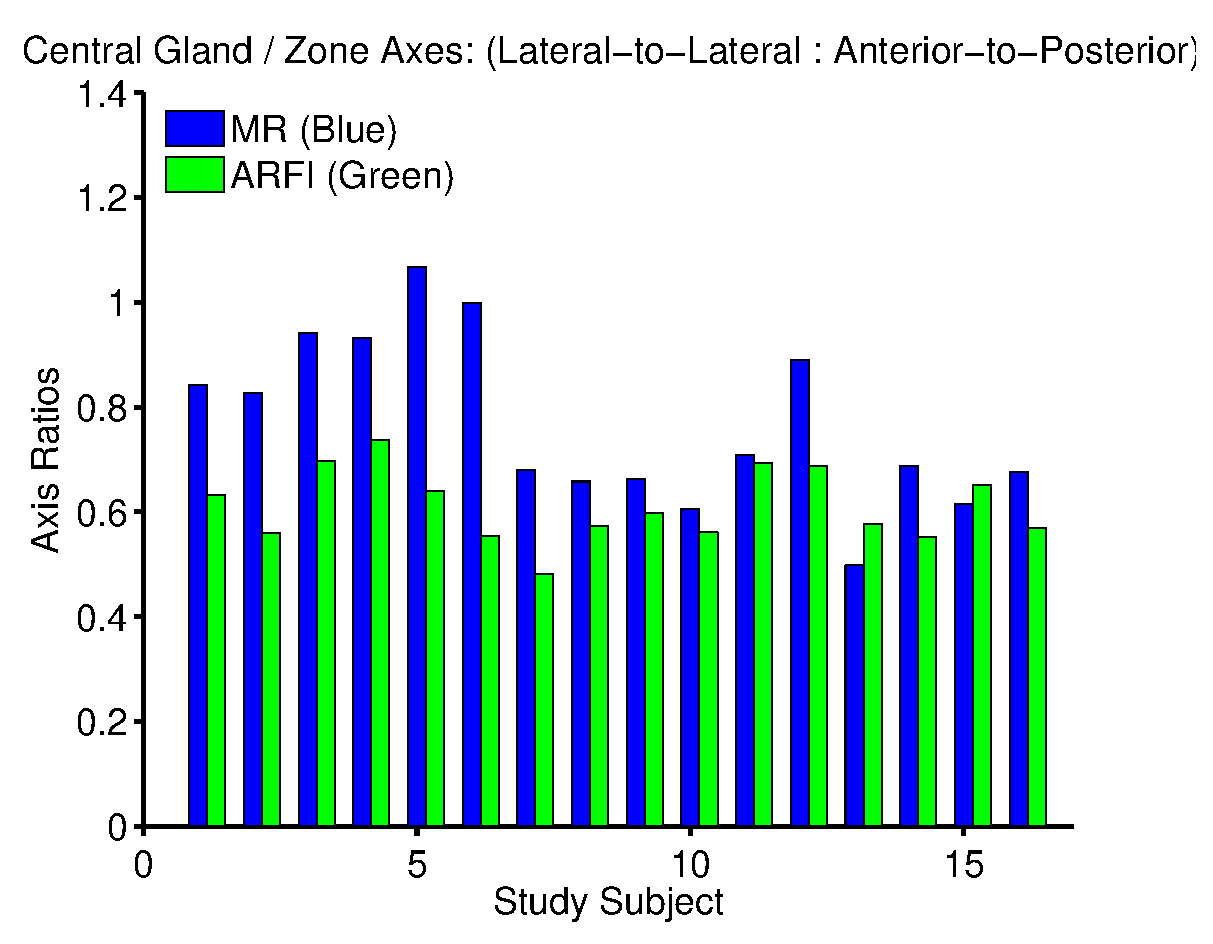
\includegraphics[width=0.3\linewidth]{figs/mr_arfi_central_axes3} \\
(a) & (b) & (c) \\
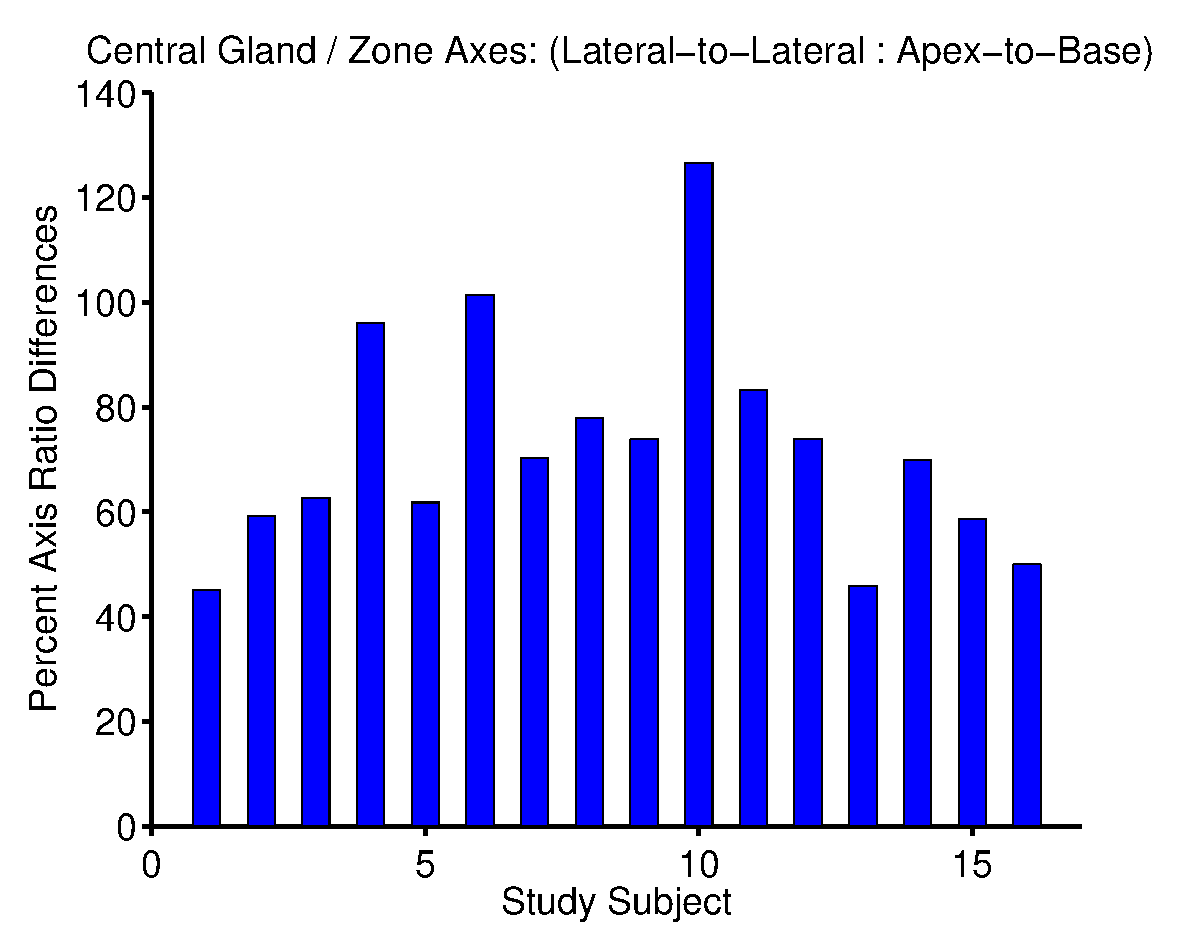
\includegraphics[width=0.3\linewidth]{figs/mr_arfi_central_over_under1.eps} &
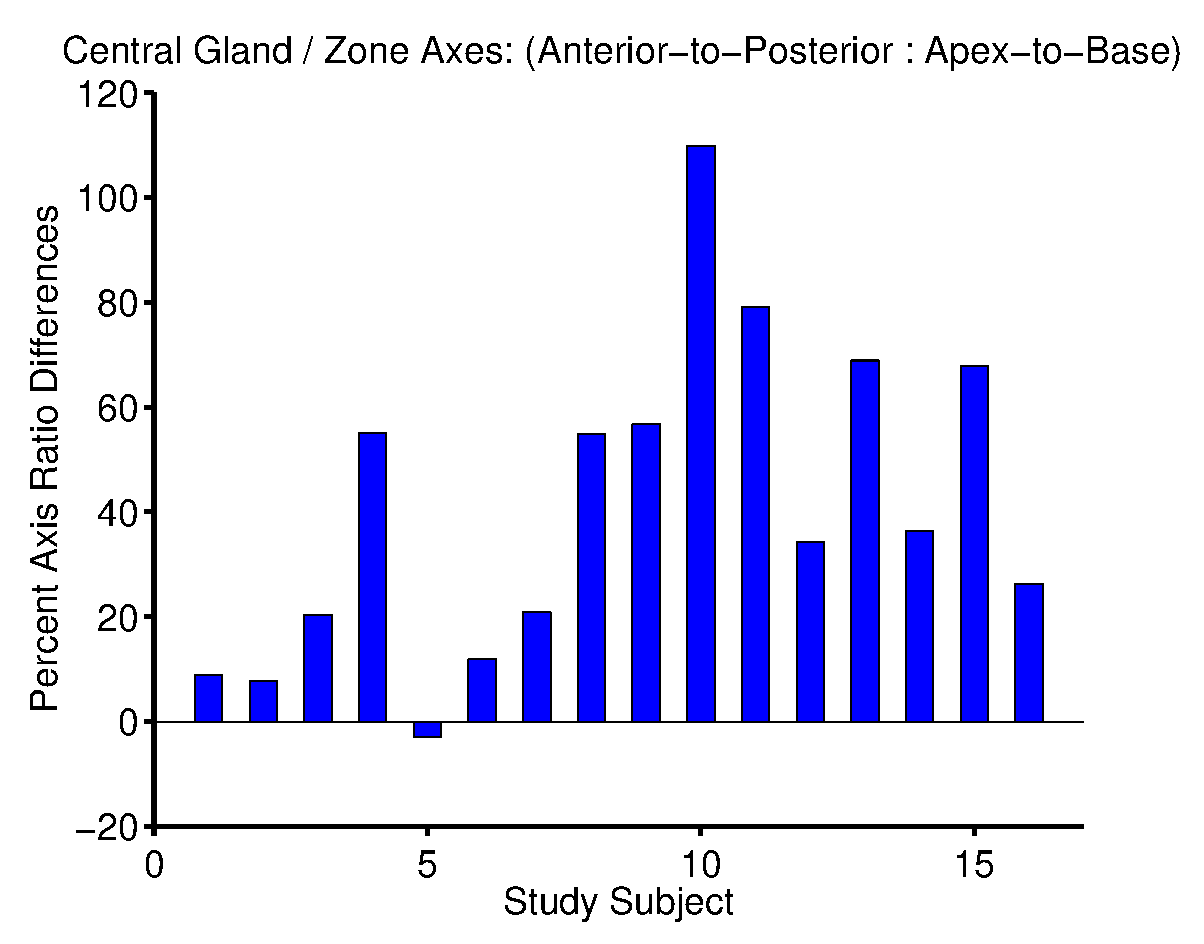
\includegraphics[width=0.3\linewidth]{figs/mr_arfi_central_over_under2.eps} &
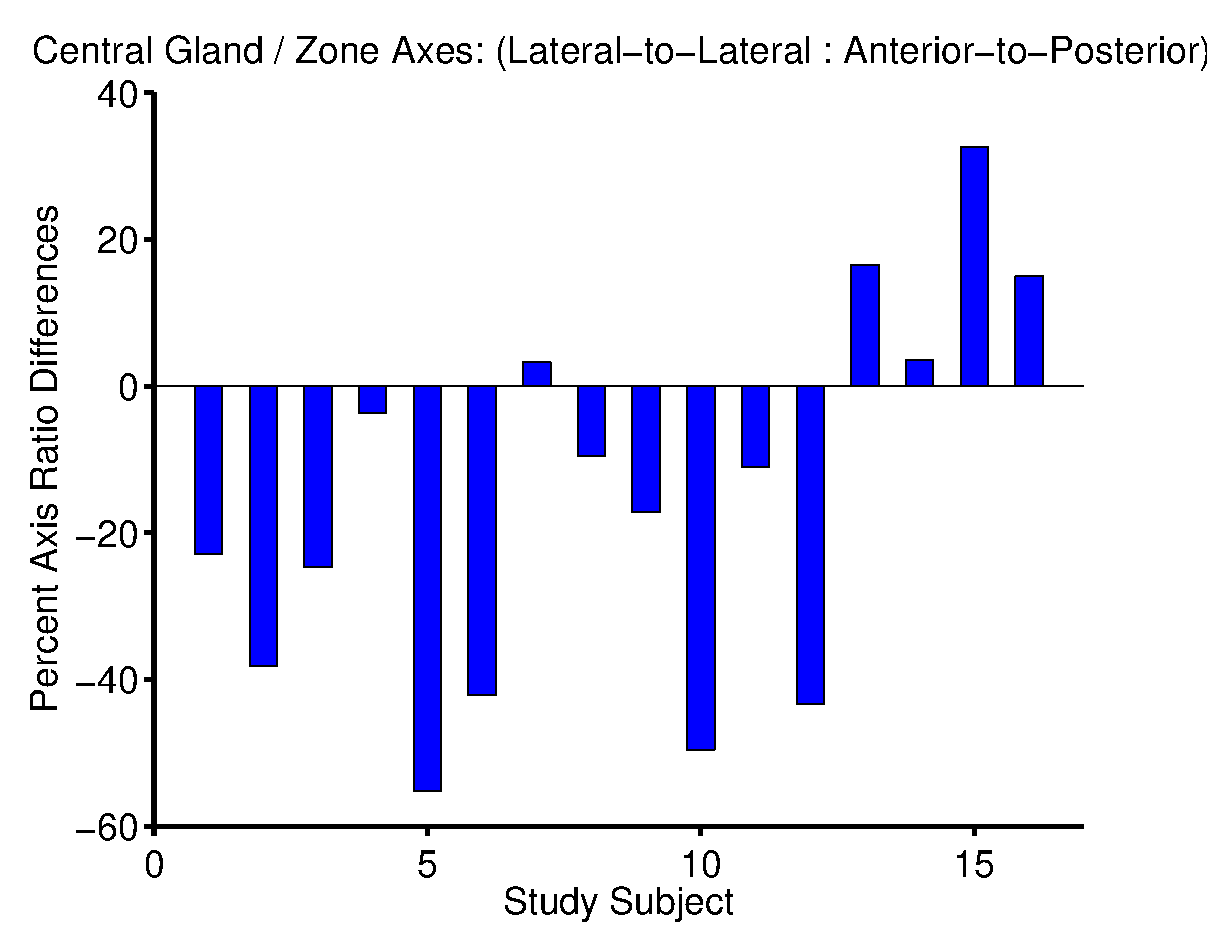
\includegraphics[width=0.3\linewidth]{figs/mr_arfi_central_over_under3.eps} \\
(a) & (b) & (c) \\
\end{tabular}
\caption{Comparison of the ratios of the three anatomic axis measurement ratios
    for T2WI MR (top row, blue) and ARFI imaging (top row, green).  The
    over/underestimation of the axis ratios between ARFI imaging and T2WI MR
    are shown in the bottom row (d-f), with mean ratio differences compiled in
    Table~\ref{tab:axis_ratio_over_under}.}
\label{fig:mr_arfi_central_axes} 
\end{figure}


%\begin{table}
\centering
\caption{Mean axis ratio differences between ARFI imaging, T2WI MR and
    pathology for the total prostate volume and central gland / zone for the
    imaging modalities.  The three axis ratios analyzed were:
    lateral-to-lateral : apex-to-base (LL:AB), anterior-to-posterio :
    apex-to-base (AP:AB), and lateral-to-lateral : anterior-to-posterior
    (LL:AP).}
\begin{tabular}{|l|l|l|l|l|} \hline
{\bf Image Modality} & {\bf Comparative Measure} & {\bf Total / Central} & {\bf Axes} & {\bf Axis Ratio Difference (\%)} \\ \hline
ARFI & MR & Total & LL:AB & 13.9 $\pm$ 22.9 \\ 
ARFI & PATH & Total & LL:AB & 39.3 $\pm$  27.6 \\ 
MR & PATH & Total & LL:AB & 24.7 $\pm$ 26.0 \\ 
ARFI & MR & Total & AP:AB & 5.2 $\pm$ 22.6 \\ 
ARFI & PATH & Total & AP:AB & 5.4 $\pm$  28.3 \\ 
MR & PATH & Total & AP:AB & 2.5 $\pm$ 26.0 \\ 
ARFI & MR & Total & LL:AP & -6.4 $\pm$ 18.3 \\ 
ARFI & PATH & Total & LL:AP & -23.3 $\pm$  17.1 \\ 
MR & PATH & Total & LL:AP & -16.5 $\pm$ 21.1 \\ 
ARFI & MR & Central & LL:AB & 12.0 $\pm$ 22.5 \\ 
ARFI & MR & Central & AP:AB & -6.1 $\pm$ 18.9 \\ 
ARFI & MR & Central & LL:AP & -13.3 $\pm$ 23.7 \\ 

\hline
\end{tabular}
\label{tab:axis_ratio_over_under}
\end{table}

